\documentclass{beamer}
\usepackage{fontspec}
\usepackage{minted}
\usepackage{tango}
\usepackage{ccicons}
\usepackage{tikz}

\mode<presentation>{\usetheme{Copenhagen}}
\title{Using static typing features for fun and profit}
\author{Marek~Kubica}
\date{6.~August~2013}
\institute{Lambda Munich}

\setsansfont{Yanone Kaffeesatz Regular}
\setmainfont{EB Garamond}
\setmonofont[Scale=0.8]{Droid Sans Mono Dotted}

\usemintedstyle{tango}
\usecolortheme{rwo}
\setbeamerfont{title}{family=\rmfamily}
%\setbeamertemplate{blocks}[rounded=false]
%\useinnertheme{default}
\setbeamertemplate{title page}[default][colsep=-0bp,rounded=false,shadow=\beamer@themerounded@shadow]

%% get rid of navigation symbols
%\setbeamertemplate{navigation symbols}{}
\beamertemplatenavigationsymbolsempty

\renewcommand{\example}[1]{{\usebeamercolor[fg]{example text} #1}}

\begin{document}

%\frame{\titlepage
%\ccby
%}

\frame{
  \titlepage
  \vfill
  \begin{center}
    \ccby{}\\[0.5ex]
    {\tiny This work is licensed under a
    \href{http://creativecommons.org/licenses/by/3.0/deed.en_US}%
    {Creative Commons Attribution 3.0 Unported License}.}
    \vspace*{-2.5ex}
  \end{center}
}


\begin{frame}{Some words upfront}
  \begin{alertblock}{Disclaimer}
    I am not a professional OCaml programmer, type theoretician etc.
  \end{alertblock}
  \pause
  \begin{alertblock}{Static typing?}
    I am neither a static typing weenie, I like dynamically typed languages
    too, so put your flamewar away (for now).
  \end{alertblock}
  \begin{exampleblock}{Comments}
    If you have comments, feel free to ask in the middle. But let's try to
    avoid big detours from the topic, alrite?
  \end{exampleblock}
\end{frame}

\begin{frame}{What is the plan?}
  \begin{itemize}
    \item Data compression support in OCaml is… kinda meh
    \item I was tasked to write some code to improve it
    \item Using OCaml FFI to interface to libarchive
    \item Thought I might as well create a better API
    \item Here to tell you about some cool things possible
  \end{itemize}
\end{frame}

\begin{frame}[fragile]{Static typing the C way}
  Let's check how C handles look like. How about checking libarchive.
  \begin{minted}[gobble=4]{c}
    __LA_DECL struct archive* archive_read_new(void);
    __LA_DECL struct archive* archive_write_new(void);
  \end{minted}
  \begin{itemize}
    \item Opaque pointer to some struct
    \item Write handles and read handles have the same type
  \end{itemize}
\end{frame}

\begin{frame}
  So, what can we do with these handles?
  \pause
  \begin{itemize}
    \item Create them
    \item Open them
    \item Read from them
    \item Write to them
    \item Close them
  \end{itemize}
  \pause
  Cool.
  \pause
  \alert{But what if we screw up?}
\end{frame}

\begin{frame}[fragile]{Segfault}
  \begin{minted}[gobble=4]{text}
    zsh: segmentation fault (core dumped)  ./errors
  \end{minted}
\end{frame}

\begin{frame}[fragile]{Double free}
\begin{minted}[fontsize=\tiny]{text}
*** Error in `./errors': double free or corruption (fasttop): 0x000000000077a010 ***
======= Backtrace: =========
/usr/lib/libc.so.6(+0x788ae)[0x7fa0c97cd8ae]
/usr/lib/libc.so.6(+0x79587)[0x7fa0c97ce587]
./errors[0x40057b]
/usr/lib/libc.so.6(__libc_start_main+0xf5)[0x7fa0c9776a15]
./errors[0x400479]
======= Memory map: ========
00400000-00401000 r-xp 00000000 fe:01 21244012                           /home/marek/lambda-munich/errors
00600000-00601000 rw-p 00000000 fe:01 21244012                           /home/marek/lambda-munich/errors
0077a000-0079b000 rw-p 00000000 00:00 0                                  [heap]
7fa0c953f000-7fa0c9554000 r-xp 00000000 fe:00 4213606                    /usr/lib/libgcc_s.so.1
7fa0c9554000-7fa0c9754000 ---p 00015000 fe:00 4213606                    /usr/lib/libgcc_s.so.1
7fa0c9754000-7fa0c9755000 rw-p 00015000 fe:00 4213606                    /usr/lib/libgcc_s.so.1
7fa0c9755000-7fa0c98f8000 r-xp 00000000 fe:00 4202529                    /usr/lib/libc-2.17.so
7fa0c98f8000-7fa0c9af8000 ---p 001a3000 fe:00 4202529                    /usr/lib/libc-2.17.so
7fa0c9af8000-7fa0c9afc000 r--p 001a3000 fe:00 4202529                    /usr/lib/libc-2.17.so
7fa0c9afc000-7fa0c9afe000 rw-p 001a7000 fe:00 4202529                    /usr/lib/libc-2.17.so
7fa0c9afe000-7fa0c9b02000 rw-p 00000000 00:00 0 
7fa0c9b02000-7fa0c9b23000 r-xp 00000000 fe:00 4203728                    /usr/lib/ld-2.17.so
7fa0c9cfa000-7fa0c9cfd000 rw-p 00000000 00:00 0 
7fa0c9d22000-7fa0c9d23000 rw-p 00000000 00:00 0 
7fa0c9d23000-7fa0c9d24000 r--p 00021000 fe:00 4203728                    /usr/lib/ld-2.17.so
7fa0c9d24000-7fa0c9d25000 rw-p 00022000 fe:00 4203728                    /usr/lib/ld-2.17.so
7fa0c9d25000-7fa0c9d26000 rw-p 00000000 00:00 0 
7fff44461000-7fff44482000 rw-p 00000000 00:00 0                          [stack]
7fff445fe000-7fff44600000 r-xp 00000000 00:00 0                          [vdso]
ffffffffff600000-ffffffffff601000 r-xp 00000000 00:00 0                  [vsyscall]
zsh: abort (core dumped)  ./errors foo
\end{minted}
\end{frame}

\begin{frame}
  What actually happens: libarchive returns \texttt{ARCHIVE\_FATAL}.\pause

  Unless you trigger a bug in libarchive. \pause
  \alert{Then it segfaults.}
\end{frame}

\begin{frame}{Lots of things can go wrong}
  \begin{itemize}
    \item Reading from handle that is not open *
    \item Writing to a read handle
    \item Not setting the options correctly (compression formats)
  \end{itemize}
  \pause
  * this actually happened
\end{frame}

\begin{frame}{Not to gripe on libarchive}
  \begin{exampleblock}{Public Service Announcement}
    libarchive is a rather well designed library. Rather idiomatic C, so don't
    think this is a deliberately bad example. It is how things are in C land.
  \end{exampleblock}

  \begin{itemize}
    \item This is an OK API for C.
    \item Fragile APIs are common in C.
  \end{itemize}

  \vspace{2ex}
  \pause
  \begin{center}
    {\Large But can we do better?}
  \end{center}
\end{frame}

\begin{frame}
  \begin{center}
    {\Huge \example{Yes}}\\
    \pause
    {\scriptsize (obviously)}
  \end{center}
\end{frame}

\begin{frame}[fragile]{Fix up the handle types}
  How to prevent writing to read handles and reading from write handles?
  \begin{minted}[gobble=4]{ocaml}
    external read_new: unit -> archive = "ost_read_new"
    external write_new: unit -> archive = "ost_write_new"
  \end{minted}
  \pause
  Yup, create different handle types.
  \begin{minted}[gobble=4]{ocaml}
    type r = archive
    type w = (archive * write_buffer_ptr * written_ptr)
  \end{minted}
  So now we have two different types to represent handles.
\end{frame}

\begin{frame}{Archivement unlocked}
  \begin{center}
    {\Huge Type safety improved!}
  \end{center}
  But of course you aren't attending the talk for this \alert{trivial}
  epiphany. We can do this easily in C as well! Let's do better.
\end{frame}

\begin{frame}[fragile]{Our handles have states!}
  The handles always traverse some fixed states:
\begin{center}
% dot2tex --figonly states.dot
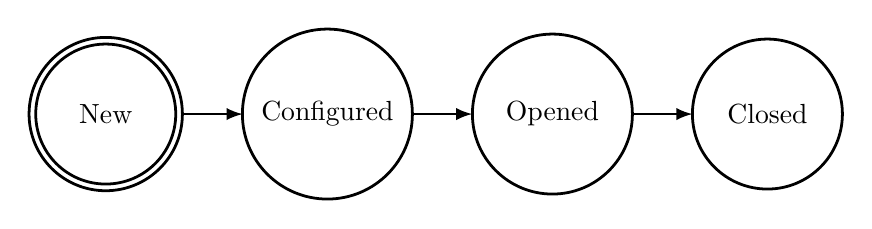
\begin{tikzpicture}[>=latex,line join=bevel,scale=0.6]
  \pgfsetlinewidth{1bp}
%%
\pgfsetcolor{black}
  % Edge: New -> Configured
  \draw [->] (92.45bp,50bp) .. controls (100.74bp,50bp) and (109.5bp,50bp)  .. (128.16bp,50bp);
  % Edge: Opened -> Closed
  \draw [->] (362.29bp,50bp) .. controls (370.61bp,50bp) and (379.33bp,50bp)  .. (398.03bp,50bp);
  % Edge: Configured -> Opened
  \draw [->] (229.9bp,50bp) .. controls (238.38bp,50bp) and (247.24bp,50bp)  .. (265.9bp,50bp);
  % Node: New
\begin{scope}
  \definecolor{strokecol}{rgb}{0.0,0.0,0.0};
  \pgfsetstrokecolor{strokecol}
  \draw (46bp,50bp) ellipse (42bp and 42bp);
  \draw (46bp,50bp) ellipse (46bp and 46bp);
  \draw (46bp,50bp) node {   New};
\end{scope}
  % Node: Configured
\begin{scope}
  \definecolor{strokecol}{rgb}{0.0,0.0,0.0};
  \pgfsetstrokecolor{strokecol}
  \draw (179bp,50bp) ellipse (51bp and 51bp);
  \draw (179bp,50bp) node {Configured};
\end{scope}
  % Node: Opened
\begin{scope}
  \definecolor{strokecol}{rgb}{0.0,0.0,0.0};
  \pgfsetstrokecolor{strokecol}
  \draw (314bp,50bp) ellipse (48bp and 48bp);
  \draw (314bp,50bp) node {  Opened};
\end{scope}
  % Node: Closed
\begin{scope}
  \definecolor{strokecol}{rgb}{0.0,0.0,0.0};
  \pgfsetstrokecolor{strokecol}
  \draw (443bp,50bp) ellipse (45bp and 45bp);
  \draw (443bp,50bp) node {  Closed};
\end{scope}
%
\end{tikzpicture}
\end{center}
Couldn't we \example{encode the state} in the type somehow?
\end{frame}

\begin{frame}[fragile]{Adding state information in the type}
  We can add state. OCaml has parametrized types *:

  \begin{minted}[gobble=4]{ocaml}
    # [];;
    - : 'a list = []
    # [1];;
    - : int list = [1]
    # type 'a read_handle = ReadHandle of 'a;;
    type 'a read_handle = ReadHandle of 'a
  \end{minted}

  * if you haven't seen them, think of them kinda like generics
\end{frame}

\begin{frame}[fragile]{Aside: Open union types}
  So, now we can \example{parametrize types with other types}.

  We could create our own state types:
  \begin{minted}[gobble=4]{ocaml}
    type state = New | Configured | Opened | Closed
  \end{minted}
  \pause
  But these \alert{can't be extended} if someone wants to add a new state.
  \pause
  \vspace{2ex}

  Plus, we're lazy.
  \begin{minted}[gobble=4]{ocaml}
    [`New] [`Configured] [`Opened] [`Closed]
  \end{minted}
  Let's use open union types aka polymorphic variants.
\end{frame}

\begin{frame}
  Great, so now we can create functions that take handles of the correct state.

  e.g. a read function that only works on \texttt{[`Opened] read\_handle}.

  \pause
  \alert{Foiled again!}
  \pause

  The OCaml compiler is too smart, it knows that \texttt{[`Opened] read\_handle} is the
  same type as \texttt{[`New] read\_handle} therefore every function which takes
  the \texttt{[`Opened]} handle takes every other type too.
\end{frame}

\begin{frame}[fragile]{Enter phantoms}
  \pause
  Let's hide the actual \texttt{read\_handle} type from the compiler.

  We create a module and only say:

  \begin{minted}{ocaml}
  module Handle : sig
    type 'a r
    (* our signatures *)
    val new : unit -> [`New] r
  end = struct
    type 'a r = read_handle
    (* our functions *)
    external new : unit -> [`Open] r = "ost_read_new"
  end
  \end{minted}
\end{frame}

\begin{frame}{Achivement unlocked!}
  \begin{center}
    {\Huge Made API misuse a type error!}
  \end{center}
  [TODO Checkbox] Writing read handles disallowed
  [TODO Checkbox] Using the proper handle in an incorrect way disallowed
\end{frame}

\end{document}
